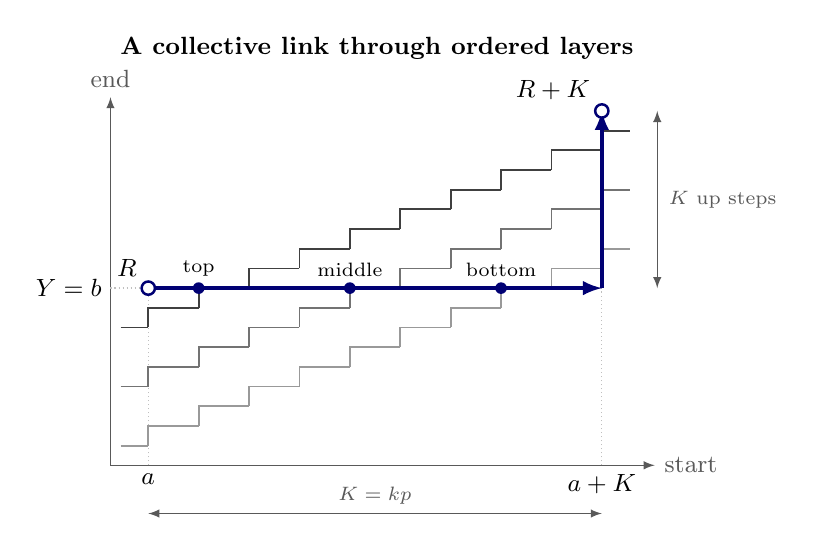
\begin{tikzpicture}[font=\small,>=latex,
  layer/.style={line width=.65pt,draw=black!55},
  connection/.style={line width=1.35pt,draw=blue!45!black},
  guide/.style={draw=black!25,densely dotted,line width=.45pt}]

  \begin{scope}[x=.64cm,y=.25cm]
    \node[anchor=west,font=\small\bfseries] at (-.75,24.2)
      {A collective link through ordered layers};
    \draw[->,black!65] (-.75,3) -- (10.05,3) node[right] {start};
    \draw[->,black!65] (-.75,3) -- (-.75,21.7) node[above] {end};
    \draw[guide] (0,3) -- (0,12);
    \draw[guide] (9,3) -- (9,12);
    \draw[guide] (-.75,12) -- (0,12);
    \node[left,inner sep=3pt] at (-.75,12) {$Y=b$};
    \node[below,inner sep=3pt] at (0,3) {$a$};
    \node[below,inner sep=3pt] at (9,3) {$a+K$};

    \foreach \c/\shade in {11/75,8/55,5/40} {
      \draw[layer,draw=black!\shade] (-.55,\c-1) -- (0,\c-1);
      \foreach \j in {0,...,8} {
        \draw[layer,draw=black!\shade]
          (\j,\j+\c-1) -- (\j,\j+\c) -- (\j+1,\j+\c);
      }
      \draw[layer,draw=black!\shade]
        (9,9+\c-1) -- (9,9+\c) -- (9.55,9+\c);
    }

    \draw[connection,->] (0,12) -- (9,12);
    \draw[connection,->] (9,12) -- (9,21);
    \foreach \j/\name in {1/top,4/middle,7/bottom} {
      \fill[blue!45!black] (\j,12) circle (2.1pt);
      \node[above,inner sep=4pt,font=\scriptsize] at (\j,12) {\name};
    }
    \filldraw[connection,fill=white,line width=.9pt] (0,12) circle (2.4pt);
    \node[above left,inner sep=4pt] at (0,12) {$R$};
    \filldraw[connection,fill=white,line width=.9pt] (9,21) circle (2.4pt);
    \node[above left,inner sep=4pt] at (9,21) {$R+K$};
    \draw[<->,black!65] (10.1,12) -- (10.1,21)
      node[midway,right,inner sep=4pt,align=left,font=\scriptsize]
      {$K$ up steps};
    \draw[<->,black!65] (0,.55) -- (9,.55)
      node[midway,above,inner sep=3pt,font=\scriptsize] {$K=kp$};
  \end{scope}
\end{tikzpicture}
